% "Станет проще"

\documentclass[a4paper,12pt]{article} % тип документа

% report, book

% Рисунки
\usepackage{graphicx}
\usepackage{wrapfig}
\usepackage{hyperref}
\usepackage[rgb]{xcolor}
\pagestyle{plain}
\usepackage{floatflt}
\usepackage{multirow}
\usepackage{lipsum}
\usepackage{amsmath, amstext}
\usepackage{siunitx}
%\usepackage{subcaption}
\usepackage{wrapfig}
\usepackage{mathrsfs}
\usepackage{adjustbox}
\usepackage{enumerate, indentfirst, float}
\usepackage{pgffor}
\usepackage{capt-of, svg}
\usepackage{array}
\usepackage{longtable}
\usepackage{csvsimple}
\usepackage{pdfpages}
\usepackage{subfigure}
\usepackage{sectsty}



%  Русский язык

\usepackage[T2A]{fontenc}			% кодировка
\usepackage[utf8]{inputenc}			% кодировка исходного текста
\usepackage[english,russian]{babel}	% локализация и переносы



% Математика
\usepackage{amsmath,amsfonts,amssymb,amsthm,mathtools} 

\usepackage{wasysym}

%Заговолок
\author{Сафиуллин Роберт	}
\title{Лабораторная работа  4.7.3\\ Поляризация}





\begin{document} % начало документа

\maketitle


\newpage

\section{Цель работы:}
  Ознакомление с методами получения и анализа поляризованного света
\\
\section{В работе используются:}
оптическая скамья с осветителем, зелёный светофильтр, два поляроида, чёрное зеркало, полированная эбонитовая пластинка, стопа стеклянных пластинок, слюдяные пластинки разной толщины, пластинки в 1/4 и 1/2 длины волны, пластинка в одну длину волны для зелёного света (пластинка чувствительного оттенка).


 
        


\section{Ход работы}

\textbf{Определение разрешённых направлений поляроидов}
\begin{figure}[H]
	\centering
	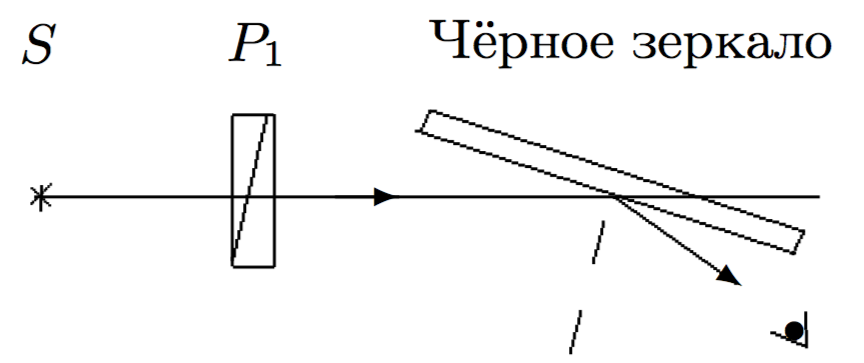
\includegraphics[width = 12 cm]{1.png}
	\caption{Определение разрешённого направления поляроида}
\end{figure}
 1) Разместили на оптической скамье осветитель S, поляроид P1 и чёрное зеркало.\\
 
 2) Поворачивая поляроид вокруг направления луча, а чёрное зеркало вокруг вертикальной оси, методом последовательных приближений добейтесь наименьшей яркости отражённого пятна.\\
 
 3) Разрешённое направление первого поляроида: 314$^o$(горизонтальное)\\
	
 4) Поставили вместо чёрного зеркала второй поляроид и определили его разрешённое направление, скрестив поляроиды\\
 
 5) Разрешённое направление второго поляроида: 259$^o$(вертикальное)\\
	

\textbf{Определение показателя преломления эбонита}
 6) Поставили на скамью вместо чёрного зеркала эбонитовую пластину и определили по лимбу угол Брюстера для эбонита\\
 7) погрешность измерения - определяется по диапазону углов, при которых пропадает отражённый свет
$$\phi_{\text{Б}} = (52\pm 7)^o$$\\

 8) Повторили измерения, добавив светофильтр Ф (зелёный).
$$\phi_{\text{Б}}^G = (53\pm 0.5)^o$$\\
 9) По углу Брюстера рассчитаем показатель преломления:\\
$$n = \tan (\phi_{\text{Б}}^G ) = 1.28\pm0.3$$
$$n = \tan (\phi_{\text{Б}} ) = 1.32\pm0.1$$
$$n^{theor} = 1.66$$

\textbf{Исследование характера поляризации света в преломлённом и отражённом от стопы лучах}
\begin{figure}[H]
	\centering
	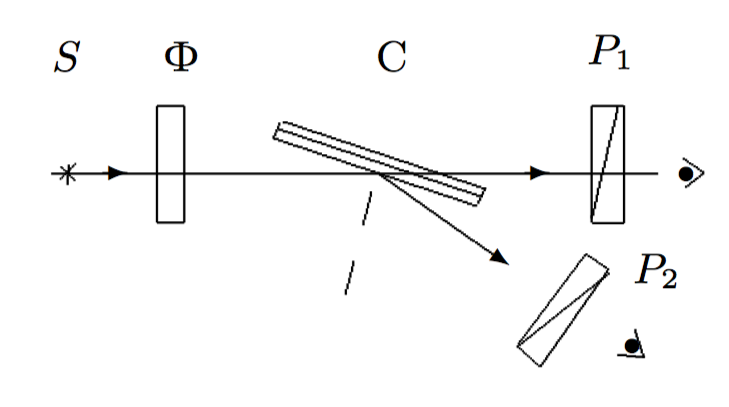
\includegraphics[height= 5 cm]{3.png}
	\caption{Исследование стопы}
\end{figure} 
 10) Поставили вместо эбонитового зеркала стопу стеклянных пластинок под углом Брюстера.\\
 11) Осветили стопу неполяризованным светом и рассматривали через поляроиды отражённый и преломлённый лучи\\
 12) В преломленном свете поляризация вертикальная \\
  В отражённом свете поляризация  горизонтальная
\\

\textbf{Определение главных направлений двоякопреломляющих пластин}

	
 13a) Поставили кристаллическую пластинку между скрещенными поляроидами.\\
 13b) Вращаем пластинку вокруг направления луча и наблюдаем за интенсивностью света, проходящего сквозь второй поляроид\\
 Главные направления пластинки: 140, 230 $^o$ совпадают с разрешёнными направлениями поляроидов - при минимуме интенсивности проходящего света
 Повторили опыт для второй пластинки, главные направления: 336 ,66 $^o$\\

\textbf{Выделения пластин $\lambda/2$ и $\lambda/4$}

 14) Добавили к схеме, изображённой на Рис. 3 (а), зелёный фильтр\\
 15) Установите разрешённое направление первого поляроида горизонтально, а главные направления исследуемой пластинки — под углом 45$^o$ к горизонтали\\
 16) С помощью второго поляроида определяем тип поляризации: \\
	 Для поляроида P1: линейная поляризация -> $\lambda/2$ \\
		Для поляроида P2: круговая поляризация -> $\lambda/4$ \\ 
	

\textbf{Определение «быстрой» и «медленной» оси в пластинке $\lambda/4$}
\begin{figure}[H]
	\centering
	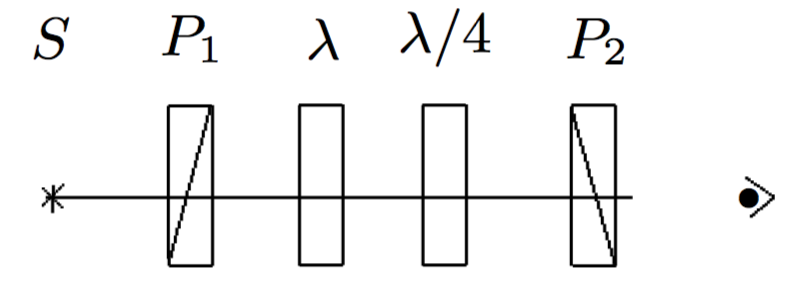
\includegraphics[width = 10 cm]{6.png}
	\caption{Определение направлений большей и меньшей скорости}
\end{figure}

 17) Поставили между скрещенными поляроидами пластинку чувствительного оттенка. Пластинка не меняет поляризацию зелёного света.\\
 18) Убрали зелёный фильтр. Стрелка имеет пурпурный цвет (так как «вырезается» зелёная часть спектра).\\
 19) Добавили к схеме пластинку $\lambda/4$, главные направления которой совпадают с главными направлениями пластины $\lambda$ и ориентированы под углом 45$^o$ к разрешённым направлениям скрещенных поляроидов.\\
 Зелёно-голубой цвет -> сопвадение «быстрых» осей -> $\lambda+\lambda/4 = 5\lambda/4$  \\(«вырезается» красная часть спектра)
	
	
\textbf{Исследование интерференции поляризованных лучей}

 20) Установиkли направление «быстрой» оси пластины $\lambda/4$ горизонтально.\\
 21) Расположили между скрещенными поляроидами мозаичную слюдяную пластинку\\
 22) При вращении пластинки наблюдаем изменение интенсивности света.\\
 23) При вращении поляроида наблюданием изменение цветов квадрата\\

\textbf{Определение направления вращения светового вектора в эллиптически поляризованной волне}

\begin{figure}[H]  
	 \centering \subfigure[]{
		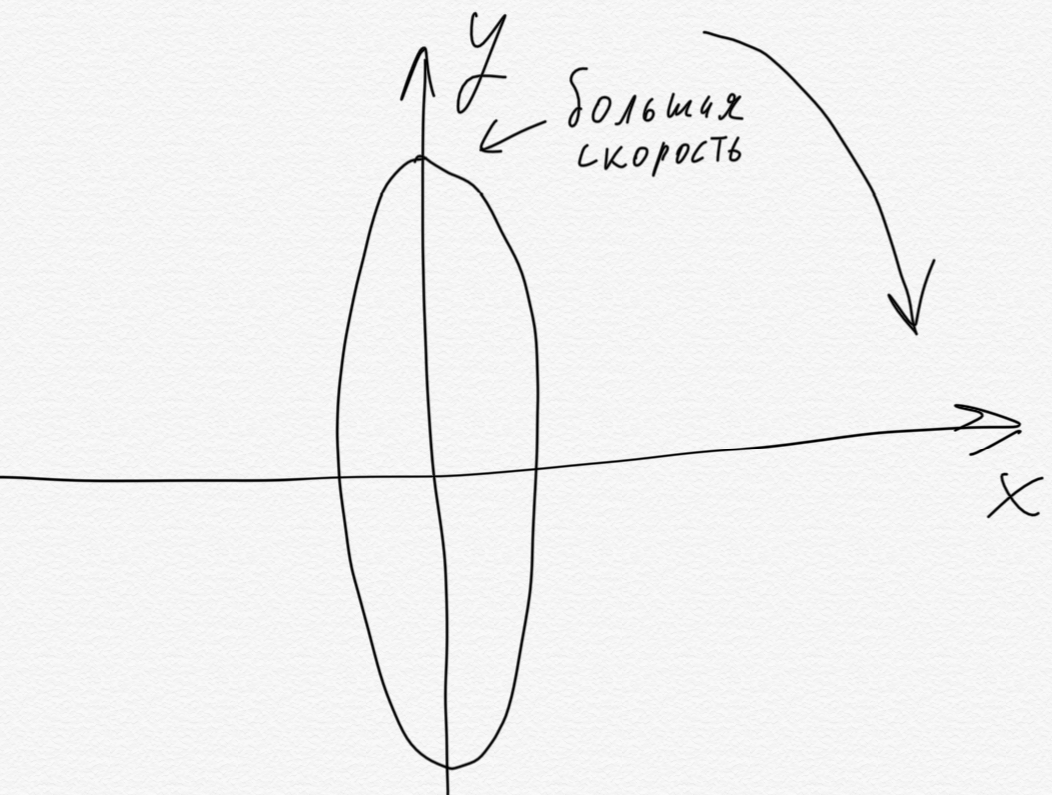
\includegraphics[width=0.3\linewidth]{8.jpeg} 
		\label{fig:a} }  
	\hspace{4ex}
	\subfigure[]{
		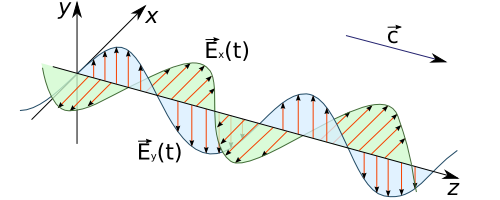
\includegraphics[width=0.55\linewidth]{polarization_elliptical.png} 
		\label{fig:b} }
	
	\caption{К определению направления вращения светового вектора} 
\end{figure}
 26) Поставили зелёный фильтр, а за ним между скрещенными поляроидами пластинку.\\
 25) Получили эллиптически-поляризованный свет. Нашли эллипс поляризации с вертикально ориентированной малой осью.





















































\end{document} % конец документа
